% Free range VHDL
% Authors: Bryan Mealy, Fabrizio Tappero
% Date: January, 2023
% URL: https://github.com/fabriziotappero/Free-Range-VHDL-book
% (C) 2018-2023 B. Mealy, F. Tappero
%
% !TEX root = master.tex
%

%%%%%%% DOCUMENT BEGIN  %%%%%%%%%%
\documentclass[13pt]{extreport}
\usepackage{style}
\begin{document}
%%%%%%%%%%%%%%%%%%%%%%%%%%%%%%%%%%

\renewcommand\contentsname{Table of Contents}
\tableofcontents

\chapter{FPGA Prototyping}
Up until now we have seen how to implement fairly basic VHDL circuits useful to execute basic tasks like count, shift left few bits, implement a decoder, etc. We however all agree that the real fun starts when your software-defined hardware becomes complex enough to actually interact with the external world.
The objective of this chapter is to present interesting real-world implementations where VHDL is in fact used to create digital circuits that have a direct application in our world. To make things even more attractive, all projects presented here will not only be explained in great detail but their synthesis and implementation on affordable FPGA-based hardware will be explained.

\section{VHDL to FPGA work flow}
Unless you are a VHDL language lawyer (a person solely interested in VHDL as a language), there will be a point in time in which you will want to take your VHDL code, synthesize it and download it on some sort of programmable hardware. This hardware could be a complex programmable logic device (CPLD) or a more interesting and sometimes very expensive field programmable gate array (FPGA).
The process of synthesizing your VHDL code into a bitstream file which can be used to program your logic device can be fairly painful and full of pitfalls. Regardless of which software tool you use the work flow that you need to follow roughly accounts of the following five fundamental steps:

\begin{description}
\item[1 - Write VHDL code.] Define a \textbf{top-level design file} and all necessary VHDL files for your design. Assign a device-specific constrain file (extension \texttt{.ucf}) that defines which pins of your FPGA/CPLD will be allocated and used. In this phase you might be interested in include already developed IP cores like, for instance, what available free of charge from OpenCores\footnote{OpenCores website: \scriptsize\url{http://www.opencores.org}}.

\item[2 - Simulate.] Test and simulate your design in a software environment that allows you to input stimulus signals to your input pins and obtain graphical representations of your design output pins. In the simulation phase it is essential to write some kind of VHDL files called \textbf{test-bench files} that defines stimulus signals and few other simulation parameters.

\item [3 - Synthesis.] Once your design is complete, you can translate your VHDL code into a lower-level description of how your digital circuit is going to be. The output of this process is a hardware-independent file that uniquely describe your design. Professionals often distribute or sell their design in this format because it guarantees the irreversibility to its original VHDL source code making it a close-source distribution.

\item [4 - Translate, Map and Place \& Route.] Decide which FPGA/CPLD device to use and translate your design into a bitstream file with extension \texttt{.bit}. This is the final product of your hard work and, in somehow, equivalent to an executable file for a personal computer. At this stage the layout of all logic elements inside the device is decided. Via specific tools it is possible to analyze and evaluate such a layout.

\item [5 - Upload to FPGA/CPLD.] Via the use of a software tool generally developed by the manufacturer of the FPGA/CPLD board that you use, upload the \texttt{.bit} file to your hardware board. This might mean upload it to the FPGA/CPLD itself or, alternatively, to the small flash memory connected to it. The second solution guarantees the functioning after your hardware experience a power cycle but it requires the bitstream file \texttt{.bit} to be previously converted into a PROM file. Your design can be distributed or sold to others via its bitstream file too. This file is of course device specific.
\end{description}

A lot more can be said about programming a FPGA/CPLD, this is especially true because a large number of software solutions exists for it. The reader is encouraged to satisfy his thirst by consulting the many tutorials available on the Internet\footnote{Xilinx ISE in-depth tutorial: \scriptsize\url{http://www.xilinx.com/support/index.htm}}.

Regarding FPGA/CPLD system, a note about time constrains deserves to be made.

\subsection{Time constrains}
During the process of synthesis it is possible to define

\subsection{Intellectual propriety cores}
Intellectually proprietary (IP) cores are complex pre-tested system-level functions that can be used to dramatically shorten development time. Some examples of IP cores are a SDRAM controller, an I2C or SPI controllers, a DVI video controller, etc.

IP cores are distributed in a few different formats, among the most popular way we can mention: 1) FPGA netlists, 2) encrypted VHDL files ,3) VHDL open-source files.

\section{Software-defined FM radio transmitter}
This section presents the implementation of a software-define FM radio transmitter in the 87.5 MHz to 108.0 MHz bandwidth. A typical FM radio will be used as a receiver.

\subsection{Motivation of this project}
When I was a young boy, my parents bought be an encyclopedia for kids that kept me very much busy during those long days in which time seemed endless. I particularly remember reading about the principle of radio waves and wireless communication and, fascinated by the subject, decided to build a crystal radio receiver. After several attempts I finally succeeded and one Sunday morning, I managed to actually hear the voice of the pope himself during the 11 o'clock mass ! That was the Italian national TV, channel one.

\begin{figure}[!b]
    \centering
	\includegraphics[width=8cm]{pics/fpgap/radio.jpg}
	\caption{Schematic representation of the simplest crystal radio. This radio has no form of power supply, it can be built in few hours and, when connected to a good antenna, it can give a remarkably clear headphone operation.}
	\label{radio}
\end{figure}

Fig.~\ref{radio} shows a similar schematic of the actual FM receiver\footnote{Crystal Radio website: \scriptsize\url{http://www.crystalradio.net/crystalplans/index.shtml}} that I implemented when I was a kid.

The thing that impressed me the most about the crystal radio is that by combining an impressively small number of fairly basic components you can actually get a piece of battery-less equipment that works. The intent here is to build a software-defined FM radio transmitter by just using an FPGA. Let us begin from some basic background information about FM radio broadcast.

\subsubsection{Frequency modulation broadcast}

To provide high-fidelity sound over a broadcast radio link a frequency-modulated (FM) broadcast signal has been standardized. The FM broadcast band falls within the VHF part of the radio spectrum: 87.5 MHz to 108.0 MHz. Radio channels are defined by a different value of the FM carrier and are spaced 100 kHz apart.

Fig.~\ref{fm_band} shows how the available bandwidth within a given channel is used.

\begin{figure}
    \centering
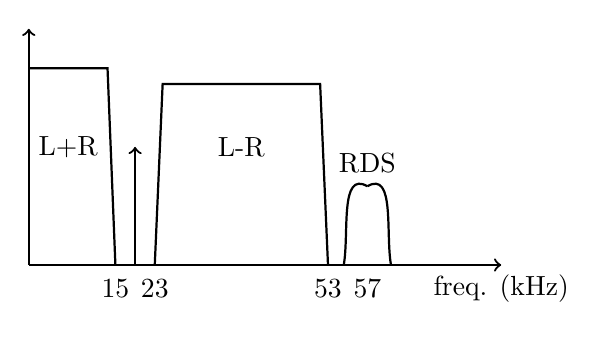
\begin{tikzpicture}
    % Draw the axis
    \draw[->,black, thick] (0,0) -- (6,0);
    \draw[->,black, thick] (0,0) -- (0,3);

    \draw[thick] (0,2.5) -- (1,2.5) -- (1.1,0);
    \draw[->,black,thick] (1.35,0) -- (1.35,1.5);
    \draw[thick] (1.6,0) -- (1.7,2.3) -- (3.7,2.3) -- (3.8,0);
    \draw[thick] (4,0) to [out=80,in=150] (4.3,1);
    \draw[thick] (4.3,1) to [out=30,in=100] (4.6,0);
    \node at (1.1,-0.3) {15};
    \node at (1.6,-0.3) {23};
    \node at (3.8,-0.3) {53};
    \node at (4.3,-0.3) {57};
    \node at (6.0,-0.3) {freq. (kHz)};
    \node at (0.5,1.5) {L+R};
    \node at (2.7,1.5) {L-R};
    \node at (4.3,1.3) {RDS};
\end{tikzpicture}
\caption{Typical channel spectrum occupancy of a FM broadcast in baseband.}
\label{fm_band}
\end{figure}

It should be noted how both left and right channels are present in their mixed form at the beginning of the channel. Also, each FM channel is equipped with a small data sub-channel, called RDS, of 1,187.5 bps on a 57 kHz subcarrier.

\subsection{FPGA-based FM transmitter}
In the following sections we will present the implementation of a FM radio transmitter using VHDL and a low-cost FPGA. In order to make this project doable by all, we have simplified the design of an FM radio transmitter to its bare minimum.

Fig.~\ref{sdr} shows the

\usetikzlibrary{circuits.ee.IEC} % electric circuit symbols library
\begin{figure}
    \centering
\begin{tikzpicture}[scale=0.7, circuit ee IEC]
    % Draw the axis
    \draw[thick] (0,0) -- (1,0)-- (1,1)-- (0,1)-- (0,0);
    \node at (5,5) {FPGA};
    \draw[thick] (0,0) -- (0,-1) node [ground, bottom] {};
    \draw (0,0) -- (0,-1) node [antenna] {};


\end{tikzpicture}
\caption{Software-defined FM radio transmitter schematic based on the Spartan 3A XC3S200A available on the XuLa board.}
\label{sdr}
\end{figure}













%%%%% DOCUMENT END  %%%%%%
\end{document}
%%%%%%%%%%%%%%%%%%%%%%%%%%
